\documentclass[11pt]{article}
\usepackage[a4paper,margin=1in]{geometry}
\usepackage{amsmath,amssymb,amsthm,bm}
\usepackage{graphicx}
\usepackage{hyperref}

\usepackage{pgfplots}
\pgfplotsset{compat=1.18}

\title{\textit{\textbf{Technical Report}}\\Distinctions and Similarities Between Log-Gaussian Cox Processes and Chi-squared Cox Processes}
\author{Tilman, Charlotte (?), Adrian (?), others (?), ...}
\date{\today}

\begin{document}
	\maketitle
	
	\section{Introduction}
	Cox processes (doubly stochastic Poisson processes) are a flexible class of models for clustered spatial point patterns. The \emph{log-Gaussian Cox process} (LGCP) is by far the most widely studied and applied, owing to its tractability and natural connection to Gaussian random fields (GRFs). 
	
	An alternative---rarely used in practice---is the \emph{chi-squared Cox process} (CSCP), in which the random intensity is given by the sum of squared Gaussian fields. Despite their similarities, the two processes induce different distributional and clustering properties. This document summarizes key properties of both models, and sketches possible avenues for publication that highlight the merits and potential uses of CSCPs.
	
	\section{Definitions}
	
	\subsection{Log-Gaussian Cox Process (LGCP)}
	An LGCP is defined by
	\[
	\Lambda(s) = \exp\{ Z(s) \}, \qquad s \in D \subset \mathbb{R}^d,
	\]
	where $Z(s)$ is a Gaussian random field with mean function $\mu(s)$ and covariance $C(s,s')$. Conditional on $\Lambda$, the point process $X$ is Poisson with intensity function $\Lambda(s)$.
	
	Key properties:
	\begin{itemize}
		\item $\mathbb{E}[\Lambda(s)] = \exp(\mu(s) + \tfrac{1}{2}\sigma^2)$.
		\item The pair correlation function is
		\[
		g(s,s') = \exp\{ C(s,s') \},
		\]
		showing that clustering strength depends exponentially on covariance. In particular, $g(0)=\exp(\sigma^2)$ can be arbitrarily large.
		\item Widely used in practice: tractable through moment properties, simulation methods, and fitting algorithms (composite likelihood, Bayesian inference, INLA).
	\end{itemize}
	
	\subsection{Chi-squared Cox Process (CSCP)}
	A CSCP is defined by
	\[
	\Lambda(s) = \sum_{i=1}^k Z_i^2(s), \qquad s \in D,
	\]
	where $\{Z_i(s)\}_{i=1}^k$ are independent Gaussian random fields with mean $\mu_i(s)$ and covariance functions $C_i(s,s')$.
	
	Key properties:
	\begin{itemize}
		\item $\mathbb{E}[\Lambda(s)] = \sum_{i=1}^k \big( \mu_i(s)^2 + \sigma_i^2 \big)$.
		\item $\mathrm{Var}[\Lambda(s)] = 2\sum_{i=1}^k \big(\sigma_i^4 + 2\mu_i^2\sigma_i^2 \big)$.
		\item The pair correlation has the form
		\[
		g(s,s') = 1 + \frac{\sum_{i=1}^k \big( \mathrm{Cov}(Z_i(s),Z_i(s')) \big)^2}{\big( \sum_{i=1}^k \sigma_i^2 + \mu_i^2 \big)^2}.
		\]
		In the symmetric zero-mean case, $g(0)=1+2/k$, so clustering strength at very short lags is bounded.
		\item Marginally, $\Lambda(s)$ follows a noncentral chi-squared distribution with $k$ degrees of freedom and noncentrality parameters $\mu_i^2/\sigma_i^2$. These marginals have lighter (exponential) tails compared to the lognormal marginals of an LGCP.
	\end{itemize}
	
	\section{Similarities and Differences}
	
	\subsection*{Similarities}
	\begin{itemize}
		\item Both are Cox processes driven by latent Gaussian random fields.
		\item Both induce clustering via spatial correlation in the latent fields.
		\item Both can represent multi-scale clustering when multiple latent fields with different correlation lengths are included.
		\item Both are second-order intensity reweighted stationary under suitable conditions, allowing use of summary statistics such as the pair correlation function.
	\end{itemize}
	
	\subsection*{Differences}
	\begin{itemize}
		\item \textbf{Marginals:} LGCP intensities are lognormal with heavy tails; CSCP intensities are chi-squared/gamma-like with lighter exponential tails.
		\item \textbf{Pair correlation:} For LGCP, $g(s,s') = \exp\{ C(s,s') \}$ and $g(0)$ can be arbitrarily large; for CSCP, $g(s,s')$ depends quadratically on covariance and $g(0)$ is bounded, yielding less explosive but potentially more interpretable clustering strength.
		\item \textbf{Role of $k$:} The degrees of freedom $k$ in CSCP controls variability and relative clustering. For large $k$, the CSCP intensity approaches Gaussianity by the central limit theorem, reducing to near-homogeneous Poisson behavior.
		\item \textbf{Interpretability:} In LGCP, the log-scale linear predictor is directly interpretable. In CSCP, $k$ may be viewed as the number of independent clustering mechanisms.
	\end{itemize}
	
%	\section{Illustration: Pair Correlation Functions}
	
%	To visualise the contrast, Figure~\ref{fig:gcomp} sketches the typical shapes of 
%	the pair correlation functions $g(h)$ for an LGCP and for a CSCP with two components. 
%	For the LGCP, $g(h)=\exp\{\sigma^2 \rho(h)\}$ grows exponentially with the covariance, 
%	so $g(0)=\exp(\sigma^2)$ can be arbitrarily large. For the CSCP, 
%	$g(h)=1+\frac{\sum_i \sigma_i^4 \rho_i(h)^2}{(\sum_i \sigma_i^2)^2}$, so $g(0)$ is 
%	bounded (e.g.\ $1+2/k$ in the symmetric case), and the shape is additive across scales.
%	




\section{Covariance structure of the CSCP intensity field}

Let the chi-squared Cox process (CSCP) be driven by $k$ independent Gaussian random fields 
\[
Z_i(s) \sim \mathrm{GRF}\!\big(\mu_i,\, \sigma_i^2 \rho_i(\|s-s'\|)\big), 
\qquad i=1,\dots,k,
\]
where $\mu_i$ is the mean, $\sigma_i^2$ the marginal variance, and 
$\rho_i(h)$ the correlation function at spatial lag $h=\|s-s'\|$. 
The random intensity is
\[
\Lambda(s) = \sum_{i=1}^k Z_i(s)^2 .
\]

\subsection{Mean intensity}
By independence across $i$,
\[
\mathbb{E}\{\Lambda(s)\}
= \sum_{i=1}^k \mathbb{E}\{Z_i(s)^2\}
= \sum_{i=1}^k \big(\mu_i^2 + \sigma_i^2\big).
\]

\subsection{Covariance function (general case)}
For any two locations $s,s'$ with separation $h=\|s-s'\|$,
\[
\operatorname{Cov}_\Lambda(h) 
= \operatorname{Cov}\!\big(\Lambda(s), \Lambda(s')\big)
= \sum_{i=1}^k \operatorname{Cov}\!\big(Z_i(s)^2, Z_i(s')^2\big),
\]
since the fields are independent across $i$.

Applying Isserlis’ (Wick’s) theorem for fourth moments of Gaussians,
\[
\mathbb{E}[Z_i(s)^2 Z_i(s')^2]
= \mathbb{E}[Z_i(s)^2]\,\mathbb{E}[Z_i(s')^2]
+ 2\,\big(\operatorname{Cov}(Z_i(s),Z_i(s'))\big)^2.
\]

Thus
\[
\operatorname{Cov}\!\big(Z_i(s)^2,Z_i(s')^2\big)
= 2 \big(\sigma_i^2 \rho_i(h)\big)^2 \;+\; 4 \mu_i^2 \sigma_i^2 \rho_i(h).
\]

Hence the full covariance is
\[
\boxed{\;
	\operatorname{Cov}_\Lambda(h) 
	= \sum_{i=1}^k \Big[\,2 \sigma_i^4 \rho_i(h)^2 \;+\; 4 \mu_i^2 \sigma_i^2 \rho_i(h)\,\Big].
	\;}
\]

\subsection{Zero-mean special case}
If $\mu_i=0$ for all $i$, this reduces to
\[
\boxed{\;\;
	\operatorname{Cov}_\Lambda(h) = 2 \sum_{i=1}^k \sigma_i^4 \rho_i(h)^2 .
	\;\;}
\]
This case is often taken as the baseline in the literature (e.g. Møller and Waagepetersen, 2004 \cite{MW2003book}).

\subsection{Pair correlation function}
The pair correlation function is defined as
\[
g(h) \;=\; 1 + \frac{\operatorname{Cov}_\Lambda(h)}{ \big(\mathbb{E}\{\Lambda(s)\}\big)^2 }.
\]
For the zero-mean, equal-variance case with exponential correlation $\rho_i(h) = \exp(-h/\phi_i)$, 
\[
g(h)-1 \;=\; \sum_{i=1}^k b_i \, e^{-2h/\phi_i},
\qquad 
b_i = \frac{2\sigma_i^4}{\Big(\sum_{j=1}^k \sigma_j^2\Big)^2}.
\]

\subsection{Semilog transformation and scale identification}
Writing $y(h)=g(h)-1$, for two components we have
\[
y(h) = b_S e^{-2h/\phi_S} + b_L e^{-2h/\phi_L}.
\]
Taking logs,
\[
\log y(h) = \log b_S - \tfrac{2h}{\phi_S} 
+ \log\!\left(1 + \tfrac{b_L}{b_S} e^{-2h\left(\tfrac{1}{\phi_L}-\tfrac{1}{\phi_S}\right)}\right).
\]

This is a log-sum-exp form: globally curved, but in limiting regimes it becomes linear:
\begin{align*}
	\log y(h) &\approx \log b_S - \tfrac{2h}{\phi_S}, && \text{if small scale dominates},\\
	\log y(h) &\approx \log b_L - \tfrac{2h}{\phi_L}, && \text{if large scale dominates}.
\end{align*}
The crossover (“shoulder”) occurs at 
\[
h^\star = \frac{\phi_S \phi_L}{2(\phi_L - \phi_S)} 
\log\!\Big(\tfrac{b_S}{b_L}\Big).
\]

Thus, on a semilog plot of $g(h)-1$, the CSCP naturally reveals its modular structure: 
straight-line regimes with slopes $-2/\phi_S$ and $-2/\phi_L$, with the transition at $h^\star$. See Figure \ref{fig:csclgcp-semilog}.


\begin{figure}[h]
	\centering
	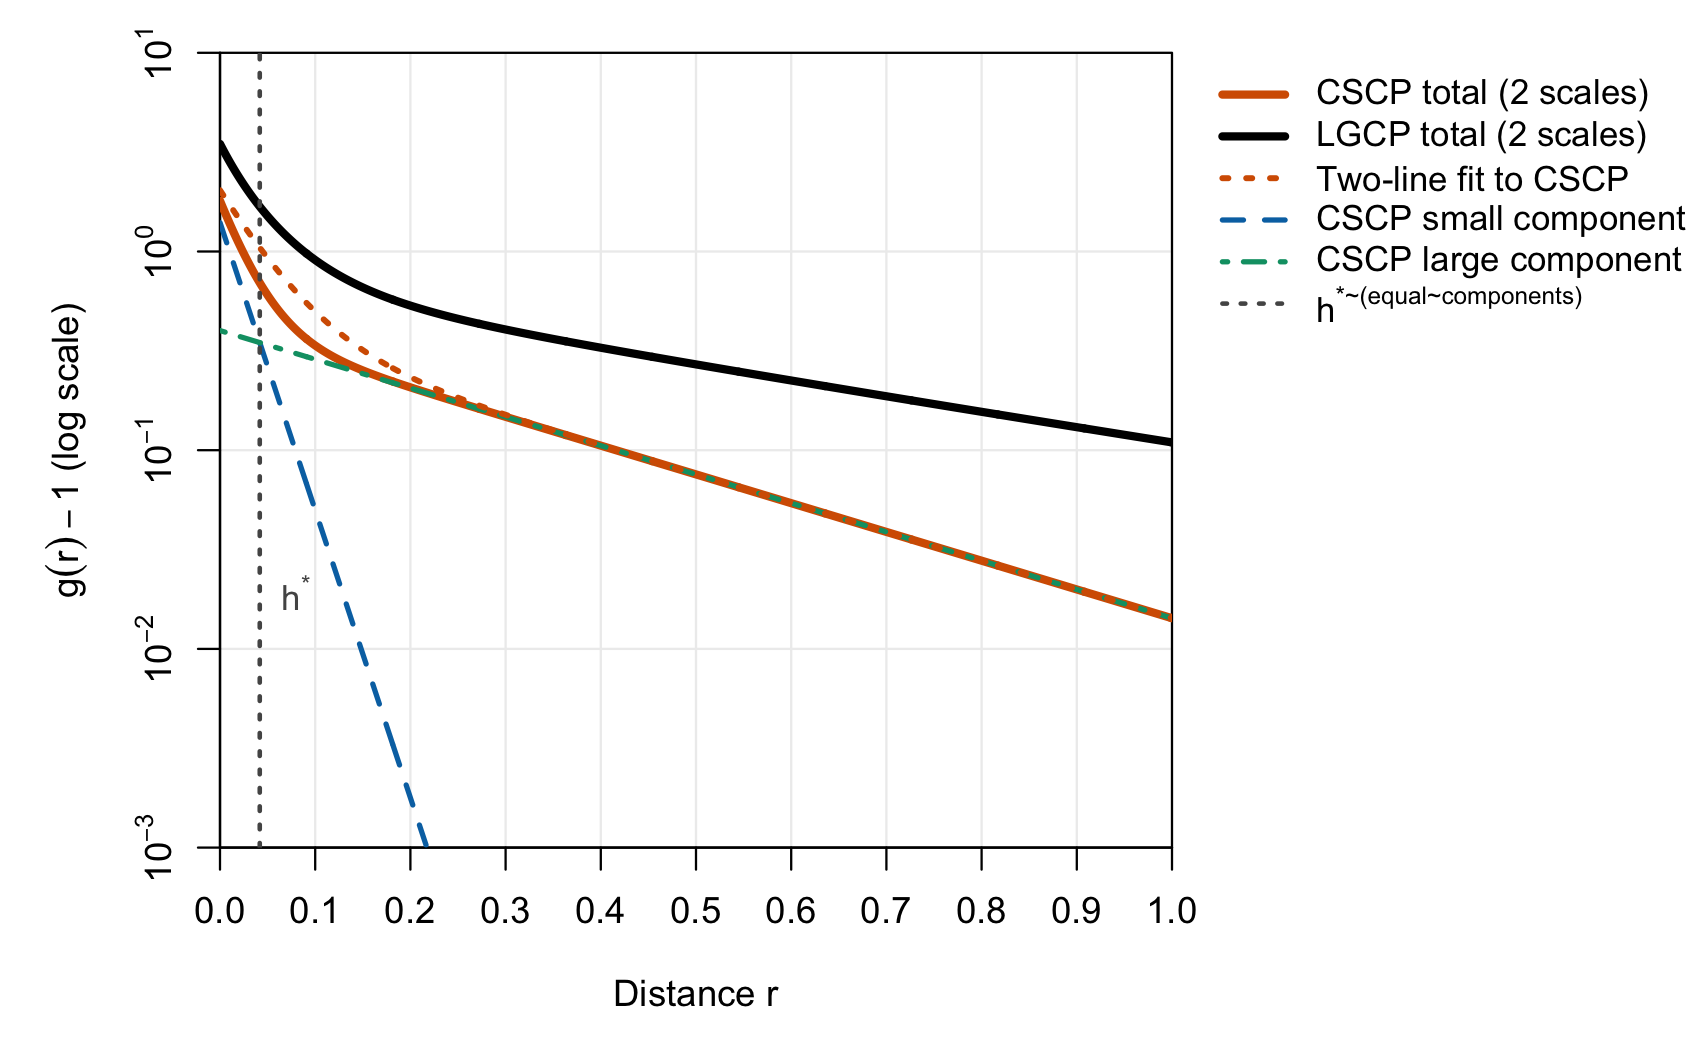
\includegraphics[width=1\textwidth]{semilog_gminus1_with_LGCP.png}
	\caption{Semilogarithmic plot of $g(h)-1$ for a two-scale CSCP. 
		Because $g(h)-1 = b_S e^{-2h/\phi_S} + b_L e^{-2h/\phi_L}$, the function is a sum of exponentials. 
		On the semilog scale, this produces two approximately linear regimes: one at small lags with slope $-2/\phi_S$ (short-range clustering), 
		and one at larger lags with slope $-2/\phi_L$ (long-range clustering). 
		The vertical marker denotes the crossover distance $h^\star$, where the two component contributions are equal. 
		This ``shoulder'' provides a natural diagnostic of the modular structure of CSCPs, 
		in contrast to LGCPs where multiple scales are entangled in the exponent and the curve remains smoothly curved.}
	\label{fig:csclgcp-semilog}
\end{figure}



\section*{Positioning relative to existing work}

The model we describe as a \emph{Chi-squared Cox process (CSCP)} is mathematically 
equivalent to the \emph{permanental process} introduced by McCullagh and M{\o}ller (2006) \cite{McCullaghMoller2006}, 
and previously foreshadowed in the boson process literature 
\cite{ShiraiTakahashi2003,ShiraiTakahashi2004}. 
Their work established the existence, joint densities, and moment properties of 
processes with intensity fields of the form 
$\Lambda(s)=\sum_{i=1}^k Z_i(s)^2$, 
with $Z_i$ Gaussian random fields. In this sense, the theoretical foundation of CSCPs 
is already solidly in place.

What seems to be missing, however, is applied development. 
In contrast to log-Gaussian Cox processes (LGCPs), 
permanental/CSCPs have seen almost no uptake in 
spatial statistics practice. I think.
In particular, several potentially valuable aspects have not been explored:
\begin{itemize}
	\item \textbf{Diagnostics and interpretability:} 
	For exponential correlations, $g(h)-1$ decomposes as a sum of exponentials, 
	which on a semilog plot reveals straight-line regimes with slopes $-2/\phi_i$. 
	This provides a natural diagnostic and a modular interpretation of multiple scales of clustering --- a feature absent in LGCPs, where scales combine inside the exponent.
	\item \textbf{Multi-scale modelling:} 
	The modular structure suggests CSCPs may offer advantages in modelling 
	both small-scale hotspots and large-scale background variation simultaneously. 
	Identifying these scales empirically and contrasting them with LGCP fits 
	has not yet been demonstrated.
	\item \textbf{Estimation and heuristics:} 
	Practical inference strategies (e.g.\ composite likelihood, minimum contrast, 
	or heuristic initialisation from pair correlation diagnostics) remain underexplored.
	\item \textbf{Applied case studies:} 
	To our knowledge, there are no published applications of CSCPs to real 
	epidemiological or ecological point pattern datasets. 
\end{itemize}

Accordingly, while the permanental/CSCP model itself is not new (some other relevant papers are \cite{WalderBishopICML2017,WalderBishopMCAP2017,Nicolis2022,Eisenbaum2008}), 
there is possibly scope for novel contributions in terms of 
applied methodology, diagnostics, and interpretability. 
Our work is positioned in this gap: to revisit CSCPs with emphasis on their 
practical merits and to provide the first systematic comparison with LGCPs in applied settings.


\bibliographystyle{plain}
\begin{thebibliography}{10}
	
	\bibitem{MW2003book}
	J.~M{\o}ller and R.~P.~Waagepetersen.
	\newblock \emph{Statistical Inference and Simulation for Spatial Point Processes}.
	\newblock Chapman \& Hall/CRC, 2003.
	Available at Routledge: \url{https://doi.org/10.1201/9780203496930}.
	
	\bibitem{McCullaghMoller2006}
	P.~McCullagh and J.~M{\o}ller.
	\newblock The permanental process.
	\newblock \emph{Advances in Applied Probability}, 38(4):873--888, 2006.
	Open version: Cambridge Core PDF \url{https://www.cambridge.org/core/services/aop-cambridge-core/content/view/1E60BA9879EAE9BBF84321FA390AFD81/S0001867800001361a.pdf/the-permanental-process.pdf}.
	
	\bibitem{ShiraiTakahashi2003}
	T.~Shirai and Y.~Takahashi.
	\newblock Random point fields associated with certain Fredholm determinants I: fermion, Poisson and boson point processes.
	\newblock \emph{Journal of Functional Analysis}, 205(2):414--463, 2003.
	Publisher page: \url{https://www.sciencedirect.com/science/article/pii/S002212360300171X}.
	
	\bibitem{ShiraiTakahashi2004}
	T.~Shirai and Y.~Takahashi.
	\newblock Random Point Fields Associated with Fermion, Boson and Other Statistics.
	\newblock In \emph{Stochastic Analysis on Large Scale Interacting Systems}, Advanced Studies in Pure Mathematics 39, pp.~345--354, 2004.
	Open PDF: \url{https://projecteuclid.org/ebooks/advanced-studies-in-pure-mathematics/Stochastic-Analysis-on-Large-Scale-Interacting-Systems/chapter/Random-Point-Fields-Associated-with-Fermion-Boson-and-Other-Statistics/10.2969/aspm/03910345.pdf}.
	
	\bibitem{WalderBishopICML2017}
	C.~J.~Walder and A.~N.~Bishop.
	\newblock Fast Bayesian Intensity Estimation for the Permanental Process.
	\newblock In \emph{Proceedings of the 34th International Conference on Machine Learning (ICML)}, 2017.
	Open PDF: \url{https://proceedings.mlr.press/v70/walder17a/walder17a.pdf}.
	
	\bibitem{WalderBishopMCAP2017}
	C.~J.~Walder and A.~N.~Bishop.
	\newblock Gamma Gaussian Cox Processes.
	\newblock \emph{Methodology and Computing in Applied Probability}, 19(2):447--465, 2017.
	
	\bibitem{Nicolis2022}
	O.~Nicolis, L.~Fernández, and J.~E. Muñoz.
	\newblock Temporal Cox Process with Folded Normal Intensity.
	\newblock \emph{Axioms}, 11(10):513, 2022.
	Open access: \url{https://www.mdpi.com/2075-1680/11/10/513}.
	
	\bibitem{Eisenbaum2008}
	N.~Eisenbaum.
	\newblock A Cox Process Involved in the Bose--Einstein Condensation.
	\newblock \emph{Annales Henri Poincaré}, 9(6):1123--1140, 2008.
	Open PDF: \url{https://link.springer.com/content/pdf/10.1007/s00023-008-0376-6.pdf}.
	
\end{thebibliography}


%\section*{Interpretation of Figure \ref{fig:csclgcp-semilog}}
%
%Figure~\ref{fig:csclgcp-semilog} illustrates a key distinction between chi-squared Cox processes (CSCPs) 
%and log-Gaussian Cox processes (LGCPs) when modelling multi-scale clustering.
%
%
%
%\paragraph{Modular structure in CSCP.}
%On a semilogarithmic plot of $g(r)-1$, each exponential component of the CSCP appears as a straight line 
%with slope $-2/\phi$. The total CSCP curve (orange solid) therefore transitions sharply between two 
%linear regimes, with the ``shoulder'' at $h^\star$ indicating the crossover from small-scale (blue dashed) 
%to large-scale (green dash-dotted) clustering. This modularity makes the underlying scales directly 
%identifiable: their ranges $\phi_S,\phi_L$ and amplitudes $b_S,b_L$ can be recovered from the slopes 
%and intercepts of straight-line fits. The orange dotted line demonstrates that a simple two-line 
%approximation captures the CSCP almost perfectly once the small-scale contribution has faded.
%
%\paragraph{Entangled structure in LGCP.}
%The LGCP curve (black solid), in contrast, remains smoothly curved. Because the covariance terms 
%combine inside the exponential, the contributions of different scales are entangled. The result is 
%greater flexibility in shape but reduced interpretability: multiple scales cannot be cleanly read off 
%from the pair correlation function. Identifying separate correlation lengths therefore requires full 
%likelihood-based estimation rather than simple diagnostic fits.
%
%\paragraph{Implications.}
%Both models capture multi-scale clustering, but the CSCP uniquely exposes its structure in a way that is 
%transparent and diagnostically useful. This ``natural modularisation'' suggests that CSCPs may offer 
%advantages when the scientific goal is to separate and interpret distinct sources of spatial dependence, 
%rather than merely to reproduce observed clustering.
%	
	
	
%	\section{Ideas for a Publication}
%	\begin{enumerate}
%		\item \textbf{Theoretical comparison:} Provide a clear account of first- and second-order properties of CSCPs, in direct analogy to LGCPs. Highlight differences in marginal tails and clustering behavior.
%		\item \textbf{Simulation study:} Illustrate how $k$, variance, and scale parameters affect intensity surfaces and point patterns, contrasting with LGCPs.
%		\item \textbf{Multi-scale modeling:} Explore whether CSCPs with a few components of differing scales can more naturally capture multi-scale clustering than LGCPs.
%		\item \textbf{Estimation methods:} Investigate feasibility of parameter estimation via composite likelihood or minimum-contrast, especially in the context of identifiability of $k$ and scale parameters.
%		\item \textbf{Applied examples:} Consider infectious disease or ecology datasets where extreme local clustering occurs atop broader structure. Argue that CSCPs may provide a better fit than LGCPs by offering bounded clustering strength and additive multi-scale decomposition.
%		\item \textbf{Connection to degrees of freedom:} Emphasize interpretability of $k$ as a ``degrees of freedom'' parameter, akin to chi-squared tests, with implications for variability control.
%	\end{enumerate}

%is there a setting where the probability of a point appearing is related to the square of a normal random variable?
	
\end{document}